\chapterauthor{Jeferson J. Lima}{Departamento de Informática (DAINF) \\Universidade Tecnológica Federal do Paraná (UTFPR)}
\chapter{Conceitos Básicos}

A component part for an electronic item is
manufactured at one of three different factories, and then delivered to
the main assembly line.Of the total number supplied, factory A supplies
50\%, factory B 30\%, and factory C 20\%. Of the components
manufactured at factory A, 1\% are faulty and the corresponding
proportions for factories B and C are 4\% and 2\% respectively. A
component is picked at random from the assembly line. What is the
probability that it is faulty?
 
\section{Introdução}\label{intro}
The term reliability usually refers to the probability that a
component or system will operate satisfactorily either at any particular
instant at which it is required or for a certain length of
time. Fundamental to quantifying reliability s a knowledge of how to
define, assess and combine probabilities \cite{Bontempi2005Adaptive}. This may hinge on identifying the
form of the variability which is nherent n most processes. If all
components had a fixed known lifetime there would be no need to model
reliability.

\begin{enumerate}[1.]
\item A component part for an electronic item is
manufactured at one of three different factories.

\item A component part $x$ for an electronic item is
manufactured at one of three different factories.
\begin{enumerate}
\item A component part for an electronic item is
manufactured at one of three different factories.

\item A component part $x$ for an electronic item is
manufactured at one of three different factories.
\begin{enumerate}[iv.]
\item A component part for an electronic item is
manufactured at one of three different factories.

\item A component part $x$ for an electronic item is
manufactured at one of three different factories.

\item A component part for an electronic item is
manufactured at one of three different factories.

\item A component part 1, 2, 3, 4 for an electronic item is
manufactured at one of three different factories.

\item A component part for enumerate list of an electronic item is
manufactured at one of three different factories.

\end{enumerate}

\item A component part for an electronic item is
manufactured at one of three different factories.

\item A component part 1, 2, 3, 4 for an electronic item is
manufactured at one of three different factories.

\item A component part for enumerate list of an electronic item is
manufactured at one of three different factories.

\end{enumerate}

\item A component part for an electronic item is
manufactured at one of three different factories.

\item A component part 1, 2, 3, 4 for an electronic item is
manufactured at one of three different factories.

\item A component part for enumerate list of an electronic item is
manufactured at one of three different factories.

\end{enumerate}

\subsection{A component part}
A component part for an electronic item is
manufactured at one of three different factories, and then delivered to
the main assembly line.Of the total number supplied, factory A supplies
50\%, factory B 30\%, and factory C 20\%. Of the components
manufactured at factory A, 1\% are faulty and the corresponding
proportions for factories B and C are 4\% and 2\% respectively. A
component is picked at random from the assembly line. What is the
probability that it is faulty \cite{ilyas2004hsn}?
A component part for an electronic item is
manufactured at one of three different factories, and then delivered to
the main assembly line. Of the total number supplied, factory A supplies
50\%, factory B 30\%, and factory C 20\%. Of the components
manufactured at factory A, 1\% are faulty and the corresponding
proportions for factories B and C are 4\% and 2\% respectively. A
component is picked at random from the assembly line. What is the
probability that it is faulty?
A component part for an electronic item is
manufactured at one of three different factories, and then delivered to
the main assembly line.Of the total number supplied, factory A supplies
50\%, factory B 30\%, and factory C 20\%. Of the components
manufactured at factory A, 1\% are faulty and the corresponding
proportions for factories B and C are 4\% and 2\% respectively. A
component is picked at random from the assembly line. What is the
probability that it is faulty?

\begin{VF}
``A Process is a structured, measured set of activities designed to produce a specific output for a particular customer
or market---A process is thus a specific ordering of work activities across time and space, with a beginning, an end.
and clearly defined inputs and outputs: a structure for action.''

\VA{Thomas Davenport}{Senior Adjutant to the Junior Marketing VP}
\end{VF}


\begin{table}%1
%\noautomaticrules
\tabletitle{Now we are engaged $(a_g^a)$ $\big(a_g^a\big)$ in a great civil war, testing whether that
nation, or any nation so conceived.}%
\begin{tabular}{lccc}
\tch{Scene}    &\tch{Reg. fts.} &\tch{Hor. fts.} &\tch{Ver. fts.}\\
Ball &19, 221 &4, 598   &3, 200\\
Pepsi$^a$&46, 281 &6, 898 &5, 400\\
Keybrd$^b$   &27, 290 &2, 968 &3, 405\\
Pepsi    &14, 796 &9, 188 &3, 209\\
\end{tabular}
\end{table}

\textbf{MultiRelational $k$-Anonymity.} Most works on $k$-anonymity focus on anonymizing a single data table; however, a real-life \cite{diamantaras1996pcn} database usually contains multiple relational tables. This has proposed a privacy model called \emph{MultiR $k$-anonymity} to ensure $k$-anonymity on multiple relational tables. Their model assumes that a relational database contains a person-specific table $PT$ and a set of tables $T_1,\cdots,T_n$, where $PT$ contains a person identifier $Pid$ and some sensitive attributes, and $T_i$, for $1 \leq i \leq n$, contains some foreign keys, some attributes in $QID$, and sensitive attributes. The general privacy notion is to ensure that for each record owner $o$ contained in the join of all tables $PT \Join T_1 \Join \cdots \Join T_n$, there exists at least $k-1$ other record owners share the same $QID$ with $o$. It is important to emphasize that the $k$-anonymization is applied at the \emph{record owner} level, not at the \emph{record} level in traditional $k$-anonymity. This idea is similar to $(X,Y)$-anonymity, where $X=QID$ and $Y=\{Pid\}$.

Most works on $k$-anonymity focus on anonymizing a single data table; however, a real-life \cite{diamantaras1996pcn} database usually contains multiple relational tables. This has proposed a privacy model called \emph{MultiR $k$-anonymity} to ensure $k$-anonymity on multiple relational tables. Their model assumes that a relational database contains a person-specific table $PT$ and a set of tables $T_1,\cdots,T_n$, where $PT$ contains a person identifier $Pid$ and some sensitive attributes, and $T_i$, for $1 \leq i \leq n$, contains some foreign keys, some attributes in $QID$, and sensitive attributes. The general privacy notion is to ensure that for each record owner $o$ contained in the join of all tables $PT \Join T_1 \Join \cdots \Join T_n$, there exists at least $k-1$ other record owners share the same $QID$ with $o$. It is important to emphasize that the $k$-anonymization is applied at the \emph{record owner} level, not at the \emph{record} level in traditional $k$-anonymity. This idea is similar to $(X,Y)$-anonymity, where $X=QID$ and $Y=\{Pid\}$.

\begin{table}[b!]%2
\tabletitle[Short Table Caption]{Now we are engaged $(a_g^a)$ $\big(a_g^a\big)$ in a great civil war, testing whether that
nation, or any nation so conceived.}%}{%
\begin{tabular}{lccc}
\tch{Scene}    &\tch{Reg. fts.} &\tch{Hor. fts.} &\tch{Ver. fts.}\\
\multicolumn{4}{@{}l@{}}{\tsh{Table Head}}\\[3pt]\hline\\[-6pt]
Ball &19, 221 &4, 598   &3, 200\\
Pepsi &46, 281 &6, 898 &5, 400\\
Keybrd   &27, 290 &2, 968 &3, 405\\
Pepsi    &14, 796 &9, 188 &3, 209\\
\end{tabular}
\end{table}

% \begin{shadebox} %This doesn’t work with the pdftex engine -- see the manual.
% A component part for an electronic item is
% manufactured at one of three different factories, and then delivered to
% the main assembly line.Of the total number supplied, factory A supplies
% 50\%, factory B 30\%, and factory C 20\%. Of the components
% manufactured at factory A, 1\% are faulty and the corresponding
% proportions for factories B and C are 4\% and 2\% respectively. A
% component is picked at random from the assembly line. What is the
% probability that it is faulty?
% \end{shadebox}

In most literature on PPDP, they \cite{jolliffe2002pca} consider a more relaxed, yet more practical, notion of privacy protection by assuming limited attacker's background knowledge. Below, the term ``victim" refers to the record owner being linked. We can broadly classify linking models to two families.

\begin{extract}
A component part for an electronic item is \cite{hyvarinen2001ica}
manufactured at one of three different factories, and then delivered to
the main assembly line.Of the total number supplied, factory A supplies
50\%, factory B 30\%, and factory C 20\%. Of the components
manufactured at factory A, 1\% are faulty and the corresponding
proportions for factories B and C are 4\% and 2\% respectively.
\end{extract}


One family considers a privacy threat occurs when an attacker is able to link a record owner to a record in a published data table, to a sensitive attribute in a published data table, or to the published data table itself. We call them \emph{record linkage}, \emph{attribute linkage}, and \emph{table linkage}, respectively. In all types of linkages, we assume that the attacker knows the $QID$ of the victim. In record and attribute linkages, we further assume that the attacker knows the presence of the victim's record in the released table, and seeks to identify the victim's record and/or sensitive information from the table \cite{yao2002can}. In table linkage, the attack seeks to determine the present or absent of the victim's record in the released table. A data table is considered to privacy preserved if the table can effectively prevent the attacker from successfully performing these types of linkages on the table \cite{madden2002tta}. Sections~\ref{intro}-\ref{sec:reclinkage} study this family of privacy models.
\begin{equation}
\mbox{var}\widehat{\Delta} = \sum_{j = 1}^t \sum_{k = j+1}^t
\mbox{var}\,(\hat{\alpha}_j - \hat{\alpha}_k)  = \sum_{j = 1}^t
\sum_{k = j+1}^t \sigma^2(1/n_j + 1/n_k). \label{2delvart2}
\end{equation}


An obvious measure of imbalance is just the difference in the
number of times the two treatments are allocated
\begin{equation}
D_n = \mathcal{M}|n_A - n_B|. \label{2deffD}
\end{equation}
For rules such as deterministic allocation, for which the expected
value of this difference can be calculated, we obtain the population
value ${\cal D}_n$.

\begin{shortbox}
\Boxhead{Box Title Here}
Another family aims at achieving the \emph{uninformative principle}: The published table should provide the attacker with little additional information beyond the background knowledge. There should not be a large difference between the prior and posterior beliefs; otherwise, there is a privacy threat~\cite{jain2004ass, jolliffe2002pca}. Many privacy models in this family are designed for statistical database and do not distinguish attributes in $T$ into $QID$, but some of them could also thwart record, attribute, and table linkages. Section~\ref{intro} studies this family of privacy models.

Let $m$ be a prime number. With the addition and multiplication as
defined above, $Z_m$ is a field.
\end{shortbox}

\begin{theorem}\label{1th:Z_m}
Let $m$ be a prime number. With the addition and multiplication as
defined above, $Z_m$ is a field.
\end{theorem}

\begin{proof}
Most of the proof of this theorem is routine.  It is clear that $0\in Z_m$
and $1\in Z_m$ are the
zero element and identity element. If $a\in Z_m$ and $a\ne 0$, then $m-a$
is the additive inverse of $a$. If $a\in Z_m$ and $a\ne 0$, then the
greatest common divisor of $a$ and $m$ is 1, and hence
there exist integers $s$ and $t$ such that $sa+tm=1$. Thus $sa=1 -tm$ is
congruent to 1 modulo $m$. Let $s^*$ be the integer in $Z_m$
congruent to $s$
modulo $m$. Then we also have $s^*a\equiv 1\  \mbox{mod}\ m$. Hence $s^*$
is
the multiplicative inverse of $a$ modulo $m$. Verification of the rest of
the field properties is now routine.\end{proof}



\section{Record Linkage Model}\label{sec:reclinkage}

In the privacy attack of \emph{record linkage}, some value $qid$ on $QID$ identifies a small number of records in the released table $T$,
called a \emph{group}. If the victim's $QID$ matches the value
$qid$, the victim is vulnerable to being linked to the small
number of records in the group \cite{madden2005taq}. In this case, the attacker faces
only a small number of possibilities for the victim's record, and
with the help of additional knowledge, there is a chance that the
attacker could uniquely identify the victim's record from the
group.


%%%\begin{table}
%%%    \tabletitle{Examples for illustrating attacks}
%%%    \begin{tabular}{|c|c|c|c|}
%%%        \hline
%%%        \textbf{Job} & \textbf{Sex} & \textbf{Age} & \textbf{Disease} \\
%%%        \hline
%%%        Engineer & Male & 35 & Hepatitis \\
%%%        Engineer & Male & 38 & Hepatitis \\
%%%        Lawyer & Male & 38 & HIV \\
%%%        Writer & Female & 30 & Flu \\
%%%        Writer & Female & 30 & HIV \\
%%%        Dancer & Female & 30 & HIV \\
%%%        Dancer & Female & 30 & HIV \\
%%%        \hline
%%%    \end{tabular}
%%%    \label{table:rawpatient}
%%%\end{table}



\subsection{A component part}
A component part for an electronic item is
manufactured at one of three different factories, and then delivered to
the main assembly line.Of the total number supplied, factory A supplies
50\%, factory B 30\%, and factory C 20\%. Of the components
manufactured at factory A, 1\% are faulty and the corresponding
proportions for factories B and C are 4\% and 2\% respectively. A
component is picked at random from the assembly line. What is the
probability that it is faulty?



\begin{figure}
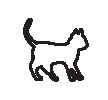
\includegraphics[width=350pt, height=200pt]{chapters/chapter1/figures/cat.eps}
%%\centerline{\epsfig{/Chapters/chapter1/figures/cat.eps,width=.8\textheight,height=.4\textwidth}}
\caption[List of figure caption goes here]{Figure caption goes here.}
\end{figure}



\begin{figure}[htb]
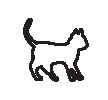
\includegraphics[width=200pt, height=200pt]{chapters/chapter1/figures/cat}
%%\centerline{\epsfig{figure=cat.eps,width=.5\textheight,height=.4\textwidth}}
\caption[Short figure caption]{Figure caption goes here. Figure caption goes here.
Figure caption goes here. Figure caption goes here. Figure caption goes here.
Figure caption goes here.}
\end{figure}





\begin{figure}
\begin{center}
\subfigure[\label{f8a}]{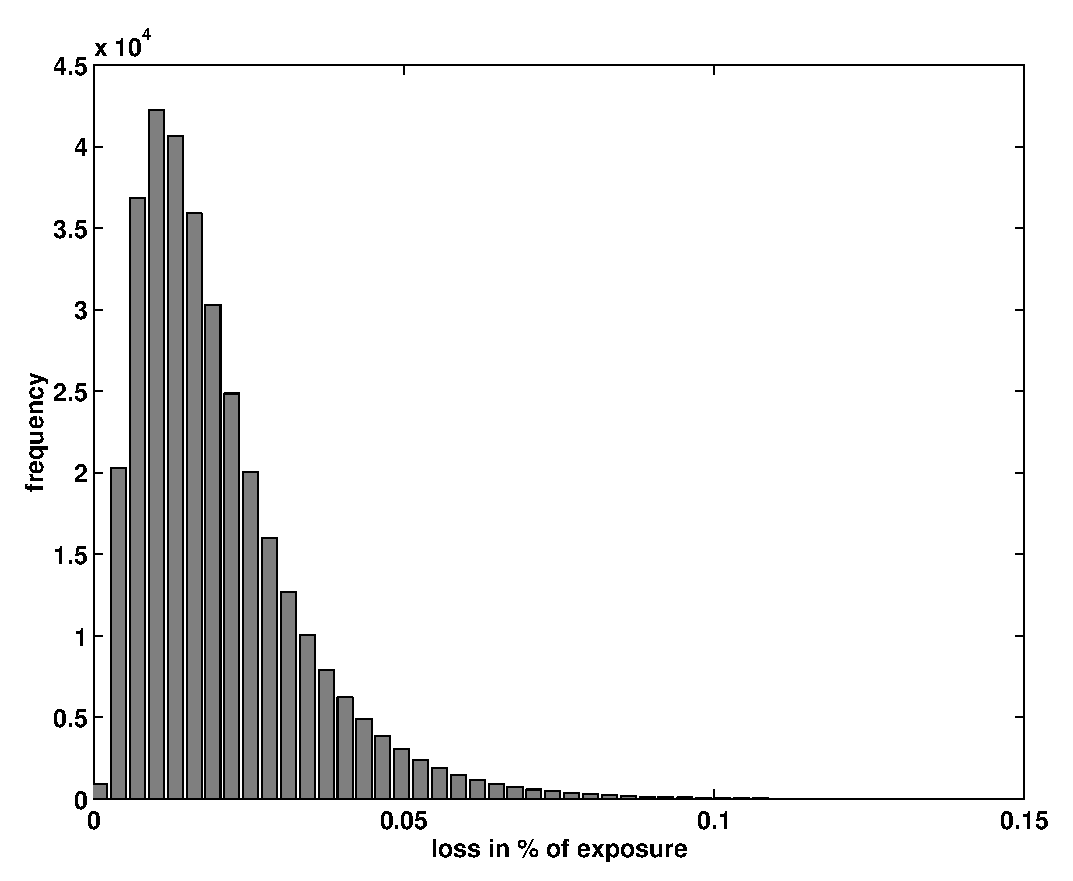
\includegraphics[angle=90,width=7cm,height=7cm,angle=-90]{chapters/chapter1/figures/Histogram.eps}}
\subfigure[\label{f8b}]{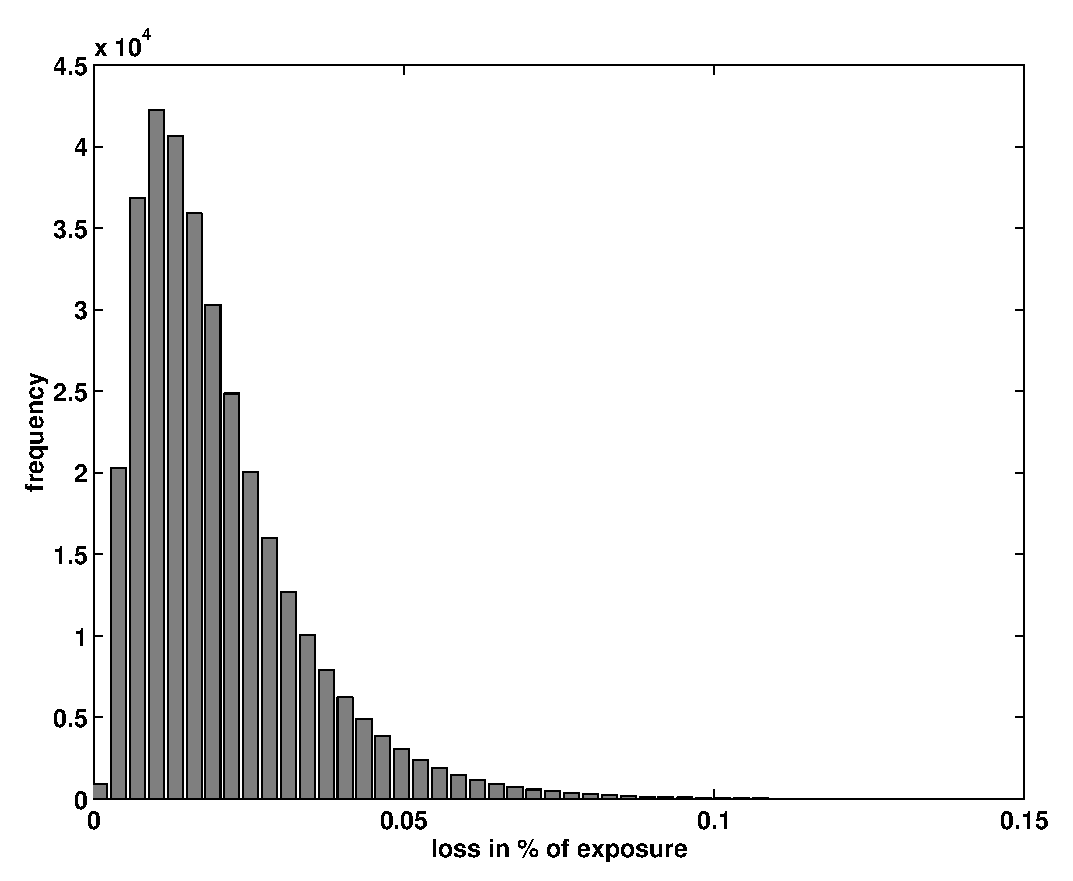
\includegraphics[angle=90,width=7cm,height=7cm,angle=-90]{chapters/chapter1/figures/Histogram.eps}}
\end{center}
\caption[The bar charts depict the different risk contributions]{The bar charts depict the different risk contributions (top: 99\% quantile, bottom: 99.9\% quantile) of the business areas of a bank. The black bars
are based on a Var/Covar approach, the white ones correspond to shortfall risk.}
\end{figure}

\subsubsection{H3 A component part }
A component part for an electronic item is
manufactured at one of three \cite{mardia1979ma} different factories, and then delivered to
the main assembly line.Of the total number supplied, factory A supplies
50\%, factory B 30\%, and factory C 20\%. Of the components
manufactured at factory A, 1\% are faulty and the corresponding
proportions for factories B and C are 4\% and 2\% respectively. A
component is picked at random from the assembly line. What is the
probability that it is faulty?


A fundamental notion \cite{yao2002can} is that of a\index{subspace}\index{vector
space!subspace of} subspace of $F^n$. Let $V$ be a nonempty subset of
$F^n$. Then $V$ is a {\it subspace} of $F^n$ provided $V$ is closed
under vector addition and scalar multiplication, that is,
\begin{enumerate}
\item[\rm (a)] For all $u$ and $v$ in $V$, $u+v$ is
also in $V$.
\item[\rm (b)] For all $u$ in $V$ and $c$ in $F$, $cu$ is
in $V$.
\end{enumerate}
Let $u$ be in the subspace $V$. Because $0u=0$,
it follows that the zero vector is in $V$. Similarly, $-u$ is in $V$
for all $u$ in $V$. A simple example of a subspace of $F^n$ is the set
of all vectors $(0,a_2,\ldots,a_n)$ with first coordinate equal to 0.
The zero vector itself is a subspace.

\begin{definition}\label{1def:linearcomb}{\rm
Let $u^{(1)},u^{(2)},\ldots,u^{(m)}$ be vectors in $F^n$, and let
$c_1,c_2,\ldots,c_m$ be scalars. Then the vector
\[c_1u^{(1)}+c_2u^{(2)}+\cdots+c_mu^{(m)}\]
is called a {\it linear combination} \index{linear combination} of $u^{(1)},u^{(2)},\ldots,u^{(m)}$.
If $V$ is a subspace of $F^n$, then $V$ is closed under vector addition and
scalar multiplication, and it follows easily by induction that a
linear combination of vectors in $V$ is also a vector in $V$. Thus
{\it subspaces
are closed under linear combinations}; in fact, this can be taken as the
defining property of subspaces.
The vectors $u^{(1)},u^{(2)},\ldots,u^{(m)}$ {\it span} $V$ \index{spanning set}
(equivalently, form a {\it spanning set} of $V$) provided every vector in
$V$
is a linear combination of $u^{(1)},u^{(2)},\ldots,u^{(m)}$. The zero
vector can be written as a linear combination of
$u^{(1)},u^{(2)},\ldots,u^{(m)}$ with all scalars equal to 0; this is a
{\it trivial linear combination}.\index{linear combination!trivial} The vectors
$u^{(1)},u^{(2)},\ldots,u^{(m)}$ are {\it linearly dependent} provided
there are scalars $c_1,c_2,\ldots,c_m$, not all of which are zero, such
that
\[c_1u^{(1)}+c_2u^{(2)}+\cdots+c_mu^{(m)}=0,\]
that is, the zero vector can be written as a {\it nontrivial linear \index{linear combination!nontrivial}
combination} of $u^{(1)},u^{(2)},\ldots,u^{(m)}$.
For example, the vectors $(1,4), (3,-1)$, and $(3,5)$ in $\Re^2$ are
linearly
dependent since
\[3(1,4)+1(3,-2)-2(3,5)=(0,0).\] Vectors are {\it linearly independent} provided  they are not linearly dependent.\index{linearly independent}
The vectors
$u^{(1)},u^{(2)},\ldots,u^{(m)}$ are a {\it basis} \index{basis} of $V$ provided they are
linearly independent and span $V$.
By an {\it ordered basis} \index{basis!ordered} we mean a basis in which the vectors of the basis are listed
in a specified order; to indicate that we have an ordered basis we write
$(u^{(1)},u^{(2)},\ldots,u^{(m)})$.
A spanning set $S$ of $V$ is a \index{spanning set!minimal} {\it minimal spanning set of $V$} provided that
each set
of vectors obtained from $S$ by removing a vector is not a spanning set
for $V$.
A linearly independent set $S$ of vectors of $V$ is a {\it maximal linearly \index{linearly independent!maximal}
independent set of vectors of $V$} provided that for each vector $w$ of
$V$ that
is not in $S$, $S\cup\{w\}$ is  linearly dependent (when this happens,
$w$ must be  a linear combination of the vectors in
$S$).\hfill{$\Box$}
}\end{definition}

In addition to matrix addition, subtraction, and multiplication, there is
one additional operation that we define now. It's perhaps the simplest of
them all. Let $A=[a_{ij}]$ be an $m$ by $n$ matrix and let $c$ be a
number \cite{hyvarinen2001ica}. Then the matrix $c\cdot A$, or simply $cA$, is the $m$ by $n$
matrix obtained by multiplying each entry of $A$ by $c$:
\[c A=[ca_{ij}].\]\index{matrix!scalar multiplication} \index{matrix!scalar multiple of}
The matrix $c A$ is called a {\it scalar multiple} of $A$.

\begin{VT1}

\VH{Think About It...}

Commonly thought of as the first modern computer, ENTAC was built in 1944. It took up more space than an 18-wheeler's
tractor trailer and weighed more than 17 Chevrolet Camaros. It consumed 140,000 watts of electricity while executing
up to 5,000 basic arithmetic operations per second. One of today's popular microprocessors, the 486, is built on a
tiny piece of silicon about the size of a dime.

\VT
With the continual expansion of capabilities, computing power will eventually exceed the capacity for human
comprehension or human control.

\VTA{The Information Revolution}{Business Week}
\end{VT1}


\section{Glossary}
\begin{Glossary}
\item[360 Degree Review] Performance review that includes feedback from superiors, peers, subordinates, and clients.
\item[Abnormal Variation] Changes in process performance that cannot be accounted for by typical day-to-day variation. Also referred to as
non-random variation.
\item[Acceptable Quality Level (AQL)] The minimum number of parts that must comply with quality standards, usually stated as a percentage.
\item[Activity] The tasks performed to change inputs into outputs.
\item[Adaptable] An adaptable process is designed to maintain effectiveness and efficiency as requirements change. The process is
deemed adaptable when there is agreement among suppliers, owners, and customers that the process will meet
requirements throughout the strategic period.
\end{Glossary}



